\chapter{\boldmath Измерение параметра \pphi в распадах \bdsth, \dbkpp в эксперименте Belle} \label{sec:bdsth}
В этой главе описано выполненное впервые модельно-независимое измерение угла Треугольника Унитарности \pphi в распадах \bdsth, \dbkpp, $h^0\in\{\pin, \eta, \etap, \omega\}$.  Метод, используемый для измерения, описан в пункте~\ref{sec:model-independent-beta} (и впервые предложен в работе автора диссертации~\cite{belle_beta_binned_dalitz}).  Для измерения использован полный интеграл светимости $711\ifb$, набранный детектором \belle вблизи резонанса \ups, соответствующий $771$ миллионам $\ups\to\bbbar$-событий.  

Для изучения фоновых процессов и выбора критериев отбора событий использованы два набора событий, полученные методом моделирования Монте-Карло: \emph{общий} и \emph{сигнальный}.  Частицы конечного состояния в обоих наборах сгенерированы с помощью пакетов \verb@EvtGen@~\cite{evtgen} и \verb@PYTHIA@~\cite{pythia}.  Излучение мягких фотонов заряженными частицами конечного состояния моделировалось с помощью пакета \verb@PHOTOS@~\cite{photos1,photos2}.  С помощью пакета \verb@GEANT4@~\cite{geant} выполнено моделирование прохождения частицами конечного состояния детектора \belle.  События моделирования сохраняются в том же формате, что экспериментальные события, содержат информацию генераторного уровня и обрабатываются аналогично экспериментальным событиям.

События общего набора моделирования сгенерированы с тем, чтобы как можно лучше воспроизвести процессы при \ep-соударениях вблизи резонанса \ups и включают большинство известных процессов вида $\ep\to\ups\to\bbbar\to X$ и $\ep\to\qqbar\to X$, $q\in\{u,d,s,c\}$.  Количество событий общего набора превосходит количество событий набранных данных приблизительно в $6$ раз.  

Для каждого события сигнального набора сгенерирован процесс $\ep\to\ups\to\bbbar$, в котором один из $B$-мезонов распадается в одно из реконструируемых конечных состояний, в то время как другой $B$-мезон распадается согласно таблице распадов, используемой для создания общего набора.

Процедура анализа событий состоит из нескольких основных этапов.  На первом этапе происходит отбор кандидатов событий \bdsth с помощью различных кинематических параметров, классификация фоновых кандидатов и применение различных алгоритмов для отбрасывания фоновых кандидатов при минимальной потере верно реконструированных (сигнальных) кандидатов, как описано в разделе~\ref{sec:event}).

На втором этапе, описанном в разделе~\ref{sec:dembc}, для каждого реконструируемого распада определяется доля сигнальных кандидатов посредством анализа двумерного распределения параметров \de и \mbc, определенных в пункте~\ref{sec:selections}.  Для выполнения такого анализа, форма сигнального и фонового распределений \de-\mbc изучаются с помощью моделирования и параметризуются соответственно функциями $p\subsig(\de,\mbc)$ и $p\subbkg(\de,\mbc)$.  Эти функции используются для определения вероятности $f_{\mathrm{sig}}^j$ того, что кандидат $j$ является сигнальным (формула~\eqref{eq:fsig_event-dependent}).  Полученные для каждого кандидата вероятности $f_{\mathrm{sig}}^j$ используются для построения функции правдоподобия при измерении угла \pphi, как описано в разделе~\ref{sec:time_likelihood}.

В главе~$2$ было показано, что для модельно-независимого получения угла \pphi необходимо выполнить разбиение фазового пространства распада \dnkpp на области.  В представленном измерении используется равномерное по фазе разбиение, основанное на модели распада из работы~\cite{belle_gamma_dalitz_model}.  Используются значения параметров \ci и \si, измеренные для этого разбиения в эксперименте CLEO~\cite{CLEO_phases}, в то время как параметры \ki мы получаем с помощью распадов \bpdpi, \dbkpp, как описано в разделе~\ref{sec:ki-meas}.

Заключительный этап анализа состоит получении параметра \pphi из распределений \dt для отобранных кандидатов методом максимального правдоподобия (раздел~\ref{sec:time_likelihood}).  Распределение по \dt для фоновых кандидатов предварительно изучается с помощью моделирования, а затем уточняется с помощью экспериментальных событий в кинематической области, не содержащей сигнальных событий.  Корректность описания фонового распределения \dt и функции разрешения по \dt для сигнальных событий проверяется посредством выполнения вспомогательного измерения времени жизни \bn-мезона в распадах \bdsth, \dbkpp. 

%\clearpage
\section{Реконструкция и отбор событий}\label{sec:event}
Для физического анализа отобраны кандидаты шести процессов \bdsth со следующими относительными вероятностями~\cite{pdg}:
\begin{equation}\label{eq:signal-modes}
 \begin{split}
  \br\left(\bdpi  \right)  &= (2.63\pm0.24)\times 10^{-4},\\
  \br\left(\bdeta \right)  &= (2.36\pm0.12)\times 10^{-4},\\
  \br\left(\bdetap\right)  &= (1.38\pm0.26)\times 10^{-4},\\
  \br\left(\bdomega\right) &= (2.53\pm0.26)\times 10^{-4},\\
  \br\left(\bdstpi\right)  &= (2.2 \pm0.6 )\times 10^{-4},\\
  \br\left(\bdsteta\right) &= (2.3 \pm0.6 )\times 10^{-4}.
 \end{split}
\end{equation}
\dn-мезон реконструируется в конечном состоянии \kspp, \kstopipi.  Вероятность перехода \dn-мезона в это конечное состояние равна~\cite{pdg}
\begin{equation}
\begin{split}
 \br(\dnkpp)\times&\br(\kstopipi) = \\
 &(2.89\pm0.08)\% \times (69.20\pm0.05)\% \approx 2\%.
\end{split}
\end{equation}

Легкие нейтральные мезоны \pin, $\eta$, \etap и $\omega$ реконструированы с распадах~\cite{pdg}
\begin{equation}\label{eq:h0-modes}
\begin{split}
 \br\left(\pigg\right)      &= (98.823 \pm 0.034)\%,\\
 \br\left(\etagg\right)     &= (39.41  \pm 0.20)\%,\\
 \br\left(\etappp\right)    &= (22.92  \pm 0.28)\%,\\
 \br\left(\omegappp\right)  &= (89.2   \pm 0.7)\%,\\
 \br\left(\etapetapp\right) &= (42.9   \pm 0.7)\%.\\
\end{split}
\end{equation}
\dst-мезоны реконструированы в конечном состоянии $\dn\pin$,  вероятность перехода в которое равна $(61.9\pm2.9)\%$~\cite{pdg}.

\subsection{Критерии отбора} \label{sec:selections}
Реконструкция заряженных $\pi$-мезонов выполнена с помощью треков, восстановленных в трековой системе детектора.  Для улучшения пространственного разрешения отбираются только треки, оставившие не менее $1$ сигнала в плоскости $r\varphi$ и не менее $2$ сигналов в плоскости $rz$ \svd.  Прицельные параметры треков относительно места взаимодействия пучков в продольном ($z$) и поперечном ($\rho$) проекциях ограничены значениями $5$~см и $2$~см, соответственно.  Поперечный импульс $p_t$ треков должен быть больше $50\mevc$ и $100\mevc$ для $\pi$-мезонов из распада \dnkpp и \hppp, соответственно, где \hn обозначает $\eta$- и $\omega$-мезоны.  Эти требования не накладывались на $\pi$-мезоны из распада \ks-мезона.

Кандидаты \ks-мезонов реконструированы в конечном состоянии $\pi^+\pi^-$.  Отбор процессов \kstopipi выполняется с помощью двух искусственных нейронных сетей.  %~\cite{phd_nakano}.  
Величина инвариантной массы \ks-кандидатов ограничена интервалом $(488.5\mevcsq,~506.5\mevcsq)$, соответствующим трем стандартным отклонениям от центрального значения.

Перечисленные ниже интервалы, ограничивающие значения инвариантных масс и других кинематических параметров, были найдены с помощью итераций с использованием событий моделирования.  Процедура выбора интервалов предполагает поочередное определение границ интервала для каждого параметра, при которых соотношение $S/\sqrt{S+B}$ принимает максимальное значение, где $S$ --- количество верно реконструированных (\emph{сигнальных}) событий и $B$ --- количество неверно реконструированных (\emph{фоновых}) событий, оставшихся после ограничения значений всех параметров соответствующими диапазонами.  Поскольку изменение диапазона для одного параметра вообще говоря влияет на выбор диапазонов для остальных параметров, процедура была выполнена в несколько итераций, до тех пор, пока границы диапазонов не перестали значительно изменяться.  %Полученные диапазоны показаны на рисунках~\ref{fig:signal_mass_ranges} и~\ref{fig:signal_dmass_ranges}.

Нейтральные $D$-мезоны реконструированы из комбинаций \ks-мезонов и треков двух противоположно заряженных частиц.  Инвариантная масса $D$-кандидатов должна быть в интервале $\left(1851.6\mevcsq, 1878.3\mevcsq\right)$ (рисунок~\ref{fig:m_d0_cut}).  

\begin{figure}[htb]
\centering
\begin{minipage}[b]{0.32\textwidth}
 \centering
  \includegraphics[width=0.99\textwidth]{m_d0_cut}
 \subcaption{}
 \label{fig:m_d0_cut}
\end{minipage}
\begin{minipage}[b]{0.32\textwidth}
 \centering
  \includegraphics[width=0.99\textwidth]{m_pi0_cut}
 \subcaption{}
 \label{fig:m_pi0_cut}
\end{minipage}
\begin{minipage}[b]{0.32\textwidth}
 \centering
  \includegraphics[width=0.99\textwidth]{m_etagg_cut}
 \subcaption{}
 \label{fig:m_etagg_cut}
\end{minipage}
\\
\begin{minipage}[b]{0.32\textwidth}
 \centering
  \includegraphics[width=0.99\textwidth]{m_etappp_cut}
 \subcaption{}
 \label{fig:m_etappp_cut}
\end{minipage}
\begin{minipage}[b]{0.32\textwidth}
 \centering
  \includegraphics[width=0.99\textwidth]{m_omega_cut}
 \subcaption{}
 \label{fig:m_omega_cut}
\end{minipage}
 \caption{События сигнального моделирования: распределения по инвариантной массе а) \dn, б) \pin, в) \etagg, г) \etappp и д) $\omega$ кандидатов.  Черные точки с ошибками показывают полученные значения, синие линии показывают аппроксимацию распределений, вертикальные красные линии показывают границы диапазонов, используемых при отборе событий для физического анализа.}
 \label{fig:signal_mass_ranges}
\end{figure}

Кандидаты \pin-мезонов реконструированы из пары фотонов с энергией не менее $40\mev$ каждый.  Инвариантная масса \pin-кандидатов должна быть внутри интервала $\left(115.7\mevcsq, 153.7\mevcsq\right)$ (рисунок~\ref{fig:m_pi0_cut}).

Кандидаты \etagg реконструированы из пары фотонов с энергией не менее $80\mev$. Инвариантная масса \etagg-кандидатов должна быть внутри интервала $\left(530.0\mevcsq, 573.7\mevcsq\right)$ (рисунок~\ref{fig:m_etagg_cut}).

Распады \hppp, где $\hn=\eta$ или $\omega$, реконструированы с использованием \pin-кандидатов с энергией не менее $200\mev$.  Инвариантная масса \etappp-кандидатов должна быть внутри интервала $\left(537.6\mevcsq, 557.4\mevcsq\right)$ (рисунок~\ref{fig:m_etappp_cut}), инвариантная масса $\omega$-кандидатов должна быть внутри интервала $\left(760.4\mevcsq, 803.9\mevcsq\right)$ (рисунок~\ref{fig:m_omega_cut}).  Косинус угла спиральности \thhel для $\omega$-кандидатов должен быть больше $0.2$.  Углом спиральности называют угол между направлением импульса \bn-мезона и нормалью к плоскости распада $\omega$-мезона в системе отсчета $\omega$-мезона.

При реконструкции распадов \etapetapp используются $\eta$-мезоны, реконструированные в конечном состоянии $\gamma\gamma$.  Разность масс $\Delta m_{\eta}$ \etap-кандидата и $\eta$-кандидата должна быть внутри интервала $\left(401.7\mevcsq, 417.7\mevcsq\right)$ (рисунок~\ref{fig:dm_etap_cut}).

\begin{figure}[htb]
\begin{minipage}[b]{0.32\textwidth}
 \centering
  \includegraphics[width=0.99\textwidth]{dm_etap_cut}
 \subcaption{}
 \label{fig:dm_etap_cut}
\end{minipage}
\begin{minipage}[b]{0.32\textwidth}
 \centering
  \includegraphics[width=0.99\textwidth]{dm_dst_pi_cut}
 \subcaption{}
 \label{fig:dm_dst_pi_cut}
\end{minipage}
\begin{minipage}[b]{0.32\textwidth}
 \centering
  \includegraphics[width=0.99\textwidth]{dm_dst_eta_cut}
 \subcaption{}
 \label{fig:dm_dst_eta_cut}
\end{minipage}
 \caption{События сигнального моделирования: распределения по разности инвариантных масс а) \etap и $\eta$ для распада $\etap\to\eta\pi^+\pi^-$, б) \dstn и \dn для распада \dstdpi и в) \dstn и \dn для распада $\dstn\to\dn\eta$.  Черные точки с ошибками показывают полученные значения, синие линии показывают аппроксимацию распределений, вертикальные красные линии показывают границы диапазонов, используемых при отборе событий для физического анализа.}
 \label{fig:signal_dmass_ranges}
\end{figure}

При реконструкции распадов $\dst\to\dn h^0$, $h^0\in\{\pin,[\gamma\gamma]_{\eta}\}$ требовалось, чтобы разность масс \dst- и \dn-кандидатов находилась в пределах диапазона $\lbr 140.2\mevcsq, 144.2\mevcsq\rbr$ (рисунки~\ref{fig:dm_dst_pi_cut} и~\ref{fig:dm_dst_eta_cut}).

Отбор \bn- и $B^{\pm}$-кандидатов выполняется с помощью двух кинематических параметров: $\de=E_B^{\cms}-E_{\mathrm{beam}}^{\cms}$ --- разности между энергией $B$-кандидата и энергией пучка в системе центра масс (\cms) и $\mbc = \sqrt{\left(E^{\cms}_{\mathrm{beam}}\right)^2-\left(p^{\cms}_{B}\right)^2}$ --- массы $B$-кандидата, посчитанной с использованием известной энергии $E^{\cms}_{\mathrm{beam}}$ пучка в \cms.  При первичном отборе $B$-кандидатов накладываются требования $-0.15\gev<\de<0.10\gev$ и $\mbc>5.2\gevcsq$.

\subsection{Выбор из нескольких кандидатов}
Некоторые события содержат несколько $B$-кандидатов, реконструированных в одном и том же конечном состоянии.  
Для дальнейшего анализа выбирается только один из них, дающий наименьшую величину параметра
\begin{equation}\label{eq:mult}
 \zeta =  \left(\frac{\dm_{\dn}}{\sigma_{m(\dn)}}\right)^2 + \left(\frac{\dm_{\hn}}{\sigma_{m(\hn)}}\right)^2 + \left(\frac{\Delta (\dm)}{\sigma_{\dm}}\right)^2,
\end{equation}
где $\dm_{\dn}$, $\dm_{\hn}$ и $\Delta(\dm)$ --- отклонения от среднего значения массы \dn-кандидата, массы \hn-кандидата и разности масс \dst- и \dn-кандидатов, соответственно,  $\sigma_i$ --- среднеквадратичные отклонения соответствующих распределений.  Если в цепочке распада нет \dstn-мезона, то третье слагаемое равно нулю.

Ожидаемое количество кандидатов в одном событии для каждой сигнальной моды и вероятность выбора сигнального кандидата изучалось с помощью моделирования (смотрите таблицу~\ref{tab:multiple_test}).  Параметр $M$, характеризующий множественность кандидатов какого-либо сигнального процесса, определен следующим образом:
\begin{equation}\label{eq:multpl}
 M = \frac{1}{N}\sum\limits_{i=0}^{N}w_i,
\end{equation}
где суммирование производится по всем событиям в выборке.  Вес $w_i$ равен нулю, если событие не содержит сигнальный кандидат,  равен $1$, если событие содержит только сигнальный кандидат и $1+n_B$, где $n_B$ --- количество фоновых кандидатов в событии.

\begin{table}[htb]
\begin{small}
  \caption{Характеристики процедуры выбора из нескольких кандидатов.  Множественность $M$ определена в уравнении \eqref{eq:multpl}.}
 \label{tab:multiple_test}
 \begin{tabular}
  { @{\hspace{0.3cm}}l@{\hspace{0.3cm}}  @{\hspace{0.3cm}}c@{\hspace{0.3cm}} @{\hspace{0.3cm}}c@{\hspace{0.3cm}} @{\hspace{0.3cm}}c@{\hspace{0.3cm}} @{\hspace{0.3cm}}c@{\hspace{0.3cm}} @{\hspace{0.3cm}}c@{\hspace{0.3cm}} @{\hspace{0.3cm}}c@{\hspace{0.3cm}} @{\hspace{0.3cm}}c@{\hspace{0.3cm}} }
  \hline\hline
 Параметр    &  \dpi  & \detagg & \detappp & \domega & \detap & \todstpi & \todsteta\\ \hline
 Множественность        & $1.03$ & $1.09$  & $1.06$   & $1.09$  & $1.08$ & $1.08$   & $1.12$ \\% \hline
 Верные решения ($\%$)  & $95.2$ & $65.1$  & $69.6$   & $66.7$  & $67.3$ & $73.8$   & $71.6$ \\% \hline
 Потеря сигнала  ($\%$) & $0.95$ & $2.78$  & $1.40$   & $2.41$  & $2.36$ & $1.72$   & $2.76$ \\
\hline\hline
 \end{tabular}
 \end{small}
\end{table}

\subsection{Определение аромата B-мезона}\label{sec:tagging}
Определение аромата помечающего \basc-мезона выполняется с помощью инклюзивного анализа частиц, не связанных с цепочкой распада сигнального $B$-мезона~\cite{flvtag}.  Информация об аромате представлена двумя параметрами: зарядом $q=\pm 1$ и чистотой $r$.  Параметр $r\in[0,1]$ определяется для каждого события и монотонно связан с вероятностью верного определения аромата: значение $r=0$ соответствует отсутствию информации об аромате, а значение $r=1$ соответствует точному определению аромата.

Значения параметра $r$ разделены на семь интервалов.  В событиях, соответствующих первому интервалу $[0,0.1)$, информация об аромате не используется.  Для остальных шести интервалов процедура определения аромата изучалась с помощью полулептонных распадов и адронных распадов с кварковым переходом $b\to c$~\cite{flvtag1,flvtag2,flvtag3}.  Для каждого интервала определена средняя вероятность неверного определения аромата $w_l$, $l\in\{1, 2,\dots, 6\}$, и их разность для распадов \bn- и \bnbar-мезонов $\Delta w_l$ (таблица~\ref{tab:wrong_tag}).

\begin{table}[htb]
\begin{small}
  \caption{Вероятность $w$ неверного определения аромата \basc и разность этих вероятностей для распадов \bn- и \bnbar-мезонов в шести диапазонах параметра $r$. Приведены значения для двух модификаций \svd.}
 \label{tab:wrong_tag}
 \begin{tabular}
  { @{\hspace{0.2cm}}l@{\hspace{0.2cm}}  @{\hspace{0.2cm}}c@{\hspace{0.2cm}} @{\hspace{0.2cm}}c@{\hspace{0.2cm}} @{\hspace{0.2cm}}c@{\hspace{0.2cm}} @{\hspace{0.2cm}}c@{\hspace{0.2cm}} @{\hspace{0.2cm}}c@{\hspace{0.2cm}} @{\hspace{0.2cm}}c@{\hspace{0.2cm}} }
  \hline\hline
  \multirow{2}{*}{Параметр} & \multicolumn{6}{c}{Диапазон $r$} \\
          & $[0.1,0.25)$ & $[0.25,0.5)$& $[0.5,0.625)$ & $[0.625,0.75)$ & $[0.75,0.875)$ & $[0.875,1)$\\ \hline
 $w$ $\svd1$ ($\%$)    & $41.9^{+0.7}_{-0.6}$ & $33.0^{+0.7}_{-0.6}$  & $23.4^{+0.7}_{-0.8}$   & $17.1^{+0.7}_{-0.6}$  & $10.0^{+0.7}_{-0.9}$ & $2.3^{+0.4}_{-0.5}$  \\% \hline
 $\Delta w$ $\svd1$ ($\%$) & $5.7\pm0.9$ & $1.3\pm0.9$  & $-1.5\pm1.0$   & $-0.1\pm0.9$  & $0.9\pm0.9$  & $0.5\pm0.6$ \\ \hline
 $w$ $\svd2$ ($\%$)    & $41.9\pm0.4$ & $31.9\pm0.3$  & $22.3^{+0.4}_{-0.3}$   & $16.3^{+0.3}_{-0.4}$  & $10.4^{+0.3}_{-0.4}$ & $2.5^{+0.2}_{-0.3}$  \\% \hline
 $\Delta w$ $\svd2$ ($\%$) & $-0.9\pm0.4$ & $1.0\pm0.4$  & $-1.1\pm0.4$   & $-1.9^{+0.4}_{-0.5}$  & $0.2\pm0.4$  & $-0.4\pm0.2$ \\% \hline
\hline\hline
 \end{tabular}
 \end{small}
\end{table}

Величина
\begin{equation*}\label{eq:effeff}
  \epseff = \sum\limits_{l=1}^6 f_l\left(1-2w_l\right)^2\approx 0.30,
\end{equation*}
где $f_l$ --- доля событий в $l$-м диапазоне, показывает эффективное уменьшение статистики из-за ошибок определения аромата \basc.

Для того, чтобы показать, что процедура отбора событий, используемая в данном анализе, не приводит к изменению приведенных значений $w_l$, была выполнена проверка.  Рисунок~\ref{fig:tag_test} показывает сравнение значений $w_l$, полученных с помощью большого количества событий сигнального моделирования процессов \bdsth с ожидаемыми значениями.  Значения согласуются в пределах статистической неопределенности.

 \begin{figure}[htb]
 \begin{minipage}[b]{0.5\textwidth}
  \centering
  \includegraphics[width=0.8\textwidth]{TagTest_w_svd1}
  \subcaption{}
 \end{minipage}
 \begin{minipage}[b]{0.5\textwidth}
  \centering
  \includegraphics[width=0.8\textwidth]{TagTest_w_svd2}
  \subcaption{}
 \end{minipage}
  \caption{Вероятность $w$ неверного определения аромата $B$-мезона в шести диапазонах значений параметра $r$ для а) $\svd1$ и б) $\svd2$. Синие круги показывают значения, полученные с помощью большого набора событий сигнального моделирования, красные квадраты показывают ожидаемые значения.}
  \label{fig:tag_test}
 \end{figure}

\subsection{Кинематическая реконструкция распадов частиц}\label{sec:kinerec}
Координаты вершин распадов $B$-мезонов определены с помощью алгоритма кинематической реконструкции, использующего треки заряженных частиц конечного состояния и информацию о расположении области взаимодействия пучков (смотрите работу~\cite{Avery} и приложение~\ref{app:kine-rec}).  Результатом работы алгоритма являются: координата $z$ вершины, оценка точности определения $\sigma_z$ этой координаты и величина $\chi^2_{\mathrm{vtx}}$, характеризующая величину сдвига траекторий заряженных частиц, необходимого для удовлетворения условию их пересечения.

Процессы \bdstarpi и \bdstaretagg не содержат заряженных частиц, вылетающих из первичной вершины распада $B$-мезона.  Координата первичной вершины для этих процессов определялась с помощью проецирования траектории $D$-мезона на область взаимодействия пучков.  Траектория $D$-мезона получена с помощью применения алгоритма кинематической реконструкции к распаду \dkpp, $\ks\to\pi^+\pi^-$.

При распаде сигнального $B$-мезона в другие рассматриваемые конечные состояния, из первичной вершины вылетают два заряженных $\pi$-мезона, рожденные в распадах $\eta$-, $\omega$ или \etap-мезонов.  Координата вершины распада $B$-мезона находится из условия пересечения треков этих $\pi$-мезонов и траектории $D$-мезона с учетом  информации о месте взаимодействия пучков.

Координата вершины \basc-мезона определяется схожим образом.  Для реконструкции этой вершины используются все треки, не задействованные в реконструкции цепочки распада сигнального $B$-мезона.

Для вершин, реконструированных с помощью нескольких треков, требуется, чтобы оценка точности определения координаты $\sigma_z$ была меньше~$0.2\mm$, а отношение величины $\chi^2_{\mathrm{vtx}}$ к количеству степеней свободы должно быть меньше~$50$.  Для вершин, реконструированных проецированием единственного трека (или траектории $D$-мезона) на область взаимодействия пучков, требуется $\sigma_z<0.5\mm$, величина $\chi^2_{\mathrm{vtx}}$ не ограничена.

Для улучшения энергетического разрешения \pin- и $\eta$-кандидатов, процедура кинематической реконструкции с требованием на инвариантную массу \pin- или $\eta$-кандидата применена к распадам $\pin\to\gamma\gamma$ и \etagg.  Аналогичная процедура, с требованием на значения инвариантных масс \dn- и \ks-кандидатов, применена к распадам \dnkpp, $\ks\to\pi^+\pi^-$.  Применение этой процедуры позволяет значительно улучшить точность определения переменных Далица распада \dnkpp (рисунок~\ref{fig:dpres}).  Кинематическая реконструкция распада \dnkpp с требованием на инвариантные массы выполняется \emph{независимо} от процедуры восстановления вершины распада $D$-мезона.  В противном случае, вершина распада $D$-мезона определяется со значительным систематическим смещением~\cite{Avery}.

\begin{figure}[htb]
 \begin{minipage}[b]{0.5\textwidth}
  \centering
  \includegraphics[width=0.9\textwidth]{dmp_raw}
  \subcaption{}
 \end{minipage}
%  \begin{minipage}[b]{0.5\textwidth}
%   \centering
%   \includegraphics[width=0.8\textwidth]{dmm_raw}
%   \subcaption{}
%  \end{minipage}
% \\
 \begin{minipage}[b]{0.5\textwidth}
  \centering
  \includegraphics[width=0.9\textwidth]{dmp_fit}
  \subcaption{}
 \end{minipage}
%  \begin{minipage}[b]{0.5\textwidth}
%   \centering
%   \includegraphics[width=0.8\textwidth]{dmm_fit}
%   \subcaption{}
%  \end{minipage}
  \caption{Распределения по ошибке измерения переменных Далица а) до и б) после применения кинематической реконструкции с требованием на значения инвариантных масс \ks- и \dn-кандидатов.}
  \label{fig:dpres}
 \end{figure}

\subsection{Классификация фоновых событий}
Мы выделяем три типа фоновых событий, различающиеся временными и кинематическими характеристиками:
\begin{enumerate}
 \item комбинаторный фон из процессов нерезонансного рождения легких кварков $\ep\to\qqbar$, $q\in\{u, d, s, c\}$.  Мы будем кратко называть эту компоненту фоном из \emph{континуума};
 \item комбинаторный фон из распадов \bbbar-пар;
 \item фон от не полностью реконструированных распадов $B$-мезонов, таких как \bpdstarrho и \bpdstarpi.%, в которых  не реконструирован заряженный $\pi$-мезон из распада $\rho^+$- или \dstp-мезона.
\end{enumerate}
%В третью фоновую компоненту дают вклад процессы \bpdstarrho и \bpdstph, в которых не реконструирован заряженный $\pi$-мезон из распада $\rho^+$- или \dstp-мезона.

Изучены также события, в которых один из сигнальных распадов~\eqref{eq:signal-modes} ошибочно реконструирован как кандидат другого сигнального распада (например, к частицам конечного состояния распада \bdpi присоединился комбинаторный \pin, и получившейся кандидат прошел критерии отбора для событий \bdstpi).  Доля таких событий не превосходит~$1\%$, что позволяет не учитывать специально их влияние при текущей точности измерения.  Более того, в большинстве случаев описанное перепутывание не приводит к ошибкам измерений, поскольку координата вершины распада сигнального $B$-мезона определяется верно (только с использованием верно реконструированного $D$-мезона), и плотность вероятности обоих распадов описывается одним и тем же выражением согласно уравнению~\eqref{eq:master-formula} (смотрите также сноску на странице~$24$).

\subsection{Подавление фона от легких кварков}
Сечение процесса $\ep\to\ups\to\bbbar$ при работе коллайдера вблизи резонанса \ups близко к $1\nb$.  Сечение нерезонансного процесса рождения пар легких кварков $\ep\to\qqbar$, $q\in\{u, d, s, c\}$ при той же энергии коллайдера примерно в три раза больше.  Легкие адроны, рожденные при адронизации легких кварков, могут сложиться при реконструкции в ложный $B$-кандидат.  Такие события составляют существенную долю фоновых событий для рассматриваемых в данной работе процессов.
 
Фоновые $B$-кандидаты из \qqbar-событий во многих случаях можно идентифицировать, используя кинематические характеристики.  Импульс легкого кварка в \cms близок к $5\gevc$, в то время как импульс $B$-мезона близок к $0.3\gevc$.  При рождении пары легких кварков (в \cms) события представляют собой две противоположно направленные адронные струи (рисунок~\ref{fig:cone}).  \bbbar-событие в \cms выглядит как изотропный распад двух $B$-мезонов (рисунок~\ref{fig:sphere}).

\begin{figure}[H]
 \begin{minipage}[b]{0.4\textwidth}
  \centering
  \includegraphics[width=0.6\textwidth]{cone}
  \subcaption{}
  \label{fig:cone}
 \end{minipage}
 \begin{minipage}[b]{0.6\textwidth}
  \centering
  \includegraphics[width=0.7\textwidth]{sphere}
  \vspace{1cm}
  \subcaption{}
  \label{fig:sphere}
 \end{minipage}
  \caption{Схематичное изображение формы событий в \cms при рождении а) пары легких кварков и б) пары $B$-мезонов на \ep-коллайдере, работающем вблизи резонанса \ups.}
  \label{fig:events_shape}
 \end{figure}

 Для выделения струйных событий используют понятие \emph{траста}~\cite{thrust}.  \emph{Ось} траста $\mathbf{T}$ определяет направление, вдоль которого сумма продольных компонент импульсов частиц максимальна.  \emph{Величина} траста $T$ определяется следующим образом:
 \begin{equation*}\label{eq:thrust}
  T = \max\limits_{\mathbf{T}}\frac{\sum\limits_i|\mathbf{p}_i\mathbf{T}|}{\sum\limits_i|\mathbf{p}_i|}.
 \end{equation*}
Для разделения \qqbar- и \bbbar-событий направление траста вычисляется отдельно для конечных частиц реконструированного \brec-мезона (\thrrec) и для остальных зарегистрированных в событии частиц (\thrasc).  Угол между \thrrec и \thrasc называют \emph{углом траста} $\theta_{\textrm{thr}}$.  Распределение по $|\cos\theta_{\textrm{thr}}|$ имеет максимум вблизи $1$ для \qqbar-событий и близко к равномерному для \bbbar-событий.

Одним из способов более полного описания кинематики события является рассмотрение моментов Фокса-Вольфрама~\cite{BARNHAM1979300,foxwolfram}
\begin{equation*}
 H_k = \sum\limits_{i,j}\frac{|\mathbf{p}_i||\mathbf{p}_j|P_k(\cos\theta_{il})}{E^2_{\textrm{vis}}},\quad k=0, 1,\dots,
\end{equation*}
где $P_k$ обозначает $k$-й полином Лежандра, $\theta_{ij}$ обозначает угол между импульсами частиц $i$ и $j$, $E_{\textrm{vis}}$ обозначает сумму измеренной в событии энергии и суммирование идет по всем частицам в событии.  Величины $R_k = H_k/H_0$ называют нормированными моментами Фокса-Вольфрама.  Нормированные моменты Фокса-Вольфрама позволяют дополнительно разделять \qqbar- и \bbbar-события.  Для двуструйных событий величина $R_k$ принимает значения близкие к $1$ ($0$) для четных (нечетных) $k$, в то время как изотропные события принимают другие значения.

В работе~\cite{sfwm} были определены \emph{модифицированные} моменты Фокса-Вольфрама.  Вместо суммирования по всем частицам в событии, было предложено различать частицы из конечного состояния \brec и все остальные частицы.  Пусть первому набору частиц соответствует индекс $s$, а второму --- индекс $o$.  Тогда можно рассматривать три набора моментов: $R_k^{so}$, $R_k^{oo}$ и $R_k^{ss}$.  Моменты $R_k^{ss}$, $R_1^{so}$ и $R_3^{so}$ исключаются из рассмотрения из-за значительной корреляции с параметрами \de и \mbc.  Остальные моменты $R_k^{ij}$ с помощью стандартной для эксперимента Belle процедуры скомбинированы в один параметр $\mcl_{\textrm{sfwm}}$, учитывающий линейные корреляции между переменными.

Направление импульса \brec для \bbbar-событий подчиняется распределению, соответствующему распаду векторного мезона на два псевдоскалярных мезона:
\begin{equation*}
 \mcp_{\bbbar}\left(\cos\theta^{\cms}_B\right)=\frac{3}{8}\left(1-\cos^2\theta^{\cms}_B\right),
\end{equation*}
где $\theta^{\cms}_B$ --- полярный угол вылета \brec в \cms. Для \qqbar-событий это распределение --- однородное.  

Для процессов \bdetap и \bdsth отбираются события с $|\cos\ththr|<0.8$ и $|\cos\theta^{\cms}_B|>0.2$.  Дальнейшее подавление \qqbar-событий выполняется с помощью отбора по параметру $\mcl_{\textrm{sfwm}}$, при котором  максимальное значение принимает отношение $S/\sqrt{S+B}$, где $S$ --- количество сигнальных событий, а $B$ --- количество фоновых событий, оставшихся после применения данного критерия.  Пороговое значение $\mcl_{\textrm{sfwm}}$ выбирается с помощью событий общего моделирования, независимо для каждого процесса.

Подавление \qqbar-событий для других четырех процессов осуществляется с помощью алгоритма AdaBoost~\cite{adaboost}, реализованного в пакете TMVA~\cite{tmva}.  В качестве входных параметров алгоритма используются:
\begin{enumerate}
 \item $|\cos\ththr|$;
 \item $|\cos\theta^{\cms}_B|$;
 \item $\mcl_{\textrm{sfwm}}$;
 \item $\ln(\chi_D^2/\ndf)$ --- логарифм величины $\chi^2$, возвращаемой процедурой кинематической реконструкции распада \dkpp, при которой масса $D$-кандидата была ограничена известным значением;
 \item Величина траста для частиц конечного состояния \brec;
 \item $\ln(E_{\gamma}^{\textrm min})$, где $E_{\gamma}^{\textrm min}$ --- минимальная энергия фотона из распада $\pin\to\gamma\gamma$ или \etagg;
 \item Только для \bdetagg: $\ln(\chi_{\eta}^2/\ndf)$ --- логарифм величины $\chi^2$, возвращаемой процедурой кинематической реконструкции распада \etagg, при которой масса $\eta$-кандидата была ограничена известным значением;
 \item Только для \bdetappp и \bdomega: величина импульса \pin;
 \item Только для \bdomega: косинус угла спиральности $\omega$-кандидата.
\end{enumerate}
На рисунке~\ref{fig:tmva_vars} показаны распределения параметров, используемых алгоритмом AdaBoost, для процесса \bdpi.  Распределения по классификационному параметру, возвращаемому алгоритмом AdaBoost для сигнальных и \qqbar-событий, показаны на рисунке~\ref{fig:tmva_output}.

\begin{figure}[htb]
   \centering
  \includegraphics[width=\textwidth]{bdt_input_pi0}
  \caption{Распределения параметров, используемых для создания классификатора, различающего события фона из континуума и сигнальные события распадов \bdpi.  Сигнальные распределения (синие сплошные гистограммы) получены с помощью сигнального моделирования.  Распределения, соответствующие \qqbar-событиям (красные заштрихованные гистограммы), получены с помощью общего моделирования.}
  \label{fig:tmva_vars}
\end{figure}

\begin{figure}[htb]
 \begin{minipage}[b]{0.5\textwidth}
  \centering
  \includegraphics[width=\textwidth]{bdt-m1}
  \subcaption{}
  \label{fig:tmva_output_pi0}
 \end{minipage}
 \begin{minipage}[b]{0.5\textwidth}
  \centering
  \includegraphics[width=0.99\textwidth]{bdt-m2}
  \subcaption{}
  \label{fig:tmva_output_etagg}
 \end{minipage}
 \\
 \begin{minipage}[b]{0.5\textwidth}
  \centering
  \includegraphics[width=0.99\textwidth]{bdt-m3}
  \subcaption{}
  \label{fig:tmva_output_petappp}
 \end{minipage}
 \begin{minipage}[b]{0.5\textwidth}
  \centering
  \includegraphics[width=0.97\textwidth]{bdt-m4}
  \subcaption{}
  \label{fig:tmva_output_omega}
  \vspace{2 mm}
 \end{minipage}
  \caption{Распределения по классификационному параметру, возвращаемому алгоритмом AdaBoost, для а) распадов \bdpi, б) \bdetagg, в) \bdetappp и г) \bdomega.  Синие сплошные гистограммы соответствуют сигнальным событиям сигнального моделирования, красные заштрихованные гистограммы соответствуют \qqbar-событиям из полного моделирования.  Вертикальные фиолетовые линии показывают пороговые значения, используемые для подавления фона от \qqbar-континуума.}
  \label{fig:tmva_output}
 \end{figure}

\clearpage
В таблице~\ref{tab:continuum_test} приведены результаты выбора пороговых значений для подавления \qqbar-событий.  Для большинства процессов доля прошедших сигнальных событий превышает~$70\%$, а доля отброшенных сигнальных событий превышает~$90\%$.
\begin{table}[htb]
\caption{Доля прошедших сигнальных событий $\varepsilon\subsig$, доля отброшенных \qqbar-событий $1-\varepsilon\subbkg$ и величина $S/\sqrt{S+B}$ при выбранном пороге подавления \qqbar-событий для каждого сигнального процесса.  Результаты получены с помощью событий моделирования.}
 \label{tab:continuum_test}
 \begin{tabular}
  { @{\hspace{0.4cm}}l@{\hspace{0.4cm}}  @{\hspace{0.4cm}}c@{\hspace{0.4cm}} @{\hspace{0.4cm}}c@{\hspace{0.4cm}}  @{\hspace{0.4cm}}c@{\hspace{0.4cm}} @{\hspace{0.4cm}}c@{\hspace{0.4cm}} @{\hspace{0.4cm}}c@{\hspace{0.4cm}} @{\hspace{0.4cm}}c@{\hspace{0.4cm}}  @{\hspace{0.4cm}}c@{\hspace{0.4cm}}} \hline\hline
 Параметр                    & $\pi^0$ & \etasubgg & \etasubppp & $\omega$ & $\eta^{\prime}$ & $D^{\star0}\pi^0$ & $D^{\star0}\eta$ \\ \hline
 %$S_{init}$                   & $635$   & $156$  & $57$    & $337$   & $28$   & $82$   & $31$   \\ \hline
 %$B_{init}$                   & $5118$  & $685$  & $195$   & $2065$  & $91$   & $239$  & $38$   \\ \hline
 %BDT (LH) cut                 & $0.27$  & $0.15$ & $0.18$  & $0.18$  & $0.56$ & $0.60$ & $0.68$ \\ \hline
 $\varepsilon_{sig}$ ($\%$)   & $67.0$  & $83.3$ & $80.3$  & $79.5$  & $72.6$ & $78.4$ & $86.5$ \\ %\hline
 $1-\varepsilon_{bkg}$ ($\%$) & $97.6$  & $91.9$ & $93.1$  & $96.7$  & $92.9$ & $91.1$ & $89.0$ \\ %\hline
 %$f_{sig}$ ($\%$)             & $77.5$  & $70.0$ & $77.2$  & $79.5$  & $72.6$ & $75.2$ & $86.3$ \\ \hline
 $S/\sqrt{S+B}$                        & $18.2$  & $9.5$  & $5.95$  & $14.6$  & $3.92$ & $6.95$ & $4.81$ \\ \hline
 \hline
 \end{tabular}
 \end{table}

\section{Изучение \de-\mbc распределений}\label{sec:dembc}
Доля сигнальных событий среди отобранных кандидатов определяется методом максимального правдоподобия из двумерного \de-\mbc распределения.  Форма сигнальных и фоновых \de-\mbc распределений изучалась с помощью моделирования.  

Была также рассмотрена возможность определения доли сигнальных событий посредством анализа одномерного \de распределения в узкой области параметра \mbc.  Преимущество такой процедуры состоит в технической простоте реализации и отсутствии необходимости учета корреляций между распределениями параметров \de и \mbc.  Статистическая неопределенность, получаемая в этом случае для доли сигнальных событий, превосходит соответствующую неопределенность, получаемую при анализе двумерных распределений, приблизительно в полтора раза.  Исходя из этого было принято решение использовать анализ двумерных распределений.
 
\subsection{Определение количества сигнальных событий}
Плотность вероятности двумерного \de-\mbc распределения для отобранных кандидатов описывается функцией вида
 \begin{equation}\label{eq:de-mbc-full-pdf}
 p\left(\de,\mbc\right) = f\subsig p\subsig+f\subcnt p\subcnt+f\subcmb p\subcmb+f\subpeak p\subpeak,\quad \sum\limits_i f_i=1,
\end{equation}
где $p\subsig$, $p\subcnt$, $p\subcmb$ и $p\subpeak$ обозначают плотности вероятности соответственно для сигнала, фона из \qqbar-континуума, комбинаторного фона от распадов $B$-мезонов и фона от не полностью реконструированных распадов $B$-мезонов.  Коэффициенты $f_i$, $i\in\{\sig, \cnt, \cmb, \peak\}$ обозначают доли соответствующих компонент среди отобранных кандидатов.  Явный вид функций приведен в приложении~\ref{sec:param}.  

Большинство параметров функции~\eqref{eq:de-mbc-full-pdf} определены с помощью событий сигнального и общего моделирования.  Чтобы минимизировать систематические ошибки, связанные с неточностью моделирования, некоторые параметры определялись из данных:
\begin{itemize}
 \item Доли $f_i$, $i\in\{\sig, \cnt, \cmb, \peak\}$, различных компонент.  Доля событий от не полностью реконструированных распадов $B$-мезонов мала для всех процессов, кроме \bdpi и \bdstpi, и не может быть определена из данных.  Для этих процессов отношение $f\subpeak/f\subcmb$ зафиксировано из событий моделирования;
 \item Коэффициенты полинома Чебышева $\cheb(\de)$ из уравнения~\eqref{eq:de-mbc-cont},  описывающие форму \de распределения комбинаторного фона от \qqbar-событий;
 \item Параметр $\de_0$ из уравнения~\eqref{eq:kuzmin-fcn}, который контролирует сдвиг вдоль оси \de плотности вероятности, описывающей события из не полностью реконструированных распадов $B$-мезонов;
 \item Координаты пика сигнального распределения на плоскости \de-\mbc.
\end{itemize}
Значения перечисленных параметров определяются методом максимального правдоподобия.

Для каждого процесса на плоскости \de-\mbc определена эллиптическая сигнальная область.  События, попавшие в эту область, используются для измерения параметра \pphi.  Количество сигнальных событий, попавших в сигнальную область, вычисляется следующим образом:
\begin{equation*}
 S = \ntot\fsig\int\limits_{\mcd\subsig}\psig(\de,\mbc)d\de\,d\mbc\equiv\ntot\fsig\isig\equiv\nsig\isig,
\end{equation*}
где $\ntot$ --- количество событий в выборке, $\nsig$ --- количество сигнальных событий в выборке, и интегрирование производится по сигнальной области $\mcd\subsig$.

% Неопределенность $\sigma_S$ в величине $S$ вычисляется следующим образом:
% \begin{equation*}
%  (\sigma_S)^2 = \left(\ntot\isig\sigma_{\fsig}\right)^2 + \nsig\isig(1-\isig),
% \end{equation*}
% где $\sigma_{\fsig}$ --- неопределенность в доле сигнальных событий \fsig.

Для проверки процедуры определения количества сигнальных событий $S$ использовались события полного моделирования, которые не были задействованы в определении параметров плотности вероятности~\eqref{eq:de-mbc-full-pdf}.  Количество событий полного моделирования, использованных для этой проверки, превосходит количество набранных в эксперименте событий примерно в два раза.  Восстановленное количество сигнальных событий согласуется с известным значением в пределах статистической неопределенности для всех процессов (смотрите таблицу~\ref{tab:purity_test}).

\begin{table}[htb]
 \caption{Результат проверки процедуры определения количества сигнальных событий в выборке, выполненной с помощью событий общего моделирования.  Количество обработанных событий превосходит количество набранных данных в два раза.  Приведены истинные значения количества сигнальных событий $S_{\textrm{true}}$ и разности $S_{\textrm{fit}}-S_{\textrm{true}}$, где $S_{\textrm{fit}}$ --- количество сигнальных событий, полученных методом максимального правдоподобия. }
 \label{tab:purity_test}
 \begin{tabular}
  { @{\hspace{0.2cm}}l@{\hspace{0.2cm}}  @{\hspace{0.2cm}}c@{\hspace{0.2cm}} @{\hspace{0.2cm}}c@{\hspace{0.2cm}}  @{\hspace{0.2cm}}c@{\hspace{0.2cm}} @{\hspace{0.2cm}}c@{\hspace{0.2cm}} @{\hspace{0.2cm}}c@{\hspace{0.2cm}} @{\hspace{0.2cm}}c@{\hspace{0.2cm}} @{\hspace{0.2cm}}c@{\hspace{0.2cm}}} \hline\hline
 Параметр                             &  \pin     & \etasubgg & \etasubppp & $\omega$   &$\eta\prime$& $D^{*0}\pi^0$ & $D^{*0}\eta$ \\ \hline
 $S_{\textrm{true}}$                  & $818$     & $248$     & $80$       & $492$      & $33$     & $154$     & $59$     \\ %\hline
 $S_{\textrm{fit}}-S_{\textrm{true}}$ & $5\pm35$  & $-9\pm21$ & $-10\pm10$ & $-25\pm34$ & $11\pm8$ & $15\pm20$ & $1\pm10$ \\ \hline
\hline
 \end{tabular}
 \end{table}

Те же события полного моделирования используются для проведения другой проверки.  После отбора событий из полученной выборки удаляются сигнальные события и выполняется анализ \de-\mbc распределений.  Количества сигнальных событий, полученные в этой процедуре, показаны в таблице~\ref{tab:purity_zero_test}.  Все величины согласуются с нулем.
 
\begin{table}[htb]
 \caption{Результат проверки процедуры определения количества сигнальных событий в выборке, выполненной с помощью событий общего моделирования.  Количество обработанных событий превосходит количество набранных данных в два раза.  Перед анализом \de-\mbc распределений из выборки были удалены сигнальных события.  Приведены полученные значения количества сигнальных событий $S_{\textrm{fit}}$ для каждого процесса. }
 \label{tab:purity_zero_test}
 \begin{tabular}
  { @{\hspace{0.2cm}}l@{\hspace{0.2cm}} @{\hspace{0.2cm}}c@{\hspace{0.2cm}} @{\hspace{0.2cm}}c@{\hspace{0.2cm}}  @{\hspace{0.2cm}}c@{\hspace{0.2cm}} @{\hspace{0.2cm}}c@{\hspace{0.2cm}} @{\hspace{0.2cm}}c@{\hspace{0.2cm}} @{\hspace{0.2cm}}c@{\hspace{0.2cm}} @{\hspace{0.2cm}}c@{\hspace{0.2cm}}} \hline\hline
 Параметр & \pin &\etasubgg  & \etasubppp & $\omega$  & $\eta\prime$ & $D^{*0}\pi^0$ & $D^{*0}\eta$ \\ \hline
 $S_{\textrm{fit}}$ &$-7\pm13$& $-10\pm9$ & $-6 \pm 3$ & $11\pm10$ & $11 \pm 5$   & $14 \pm 13$   & $5 \pm 4$    \\ \hline
\hline
 \end{tabular}
 \end{table}

Информация, полученная при анализе распределений \de-\mbc, может быть использована для вычисления вероятности $f\subsig^j$ того, что некоторый кандидат~$j$, попавший в область диаграммы Далица с индексом~$i_j$ и аромат которого определен как~$q_B^j$, является сигнальным.  Для получения вероятности~$f\subsig^j$ сначала необходимо получить ожидаемое количество сигнальных событий в области~$i_j$:
\begin{equation}
 S_j = Sn_{i_j,q^j_B},
\end{equation}
где $n_{i_j,q^j_B}$ обозначает ожидаемую долю сигнальных событий, соответствующую области $i_j$ и аромату $q_B^j$, которая может быть получена интегрированием уравнения~\eqref{eq:master-formula} по времени:
\begin{equation}\label{eq:nsig-prediction-with-tag}
   n_{i,q_B} =\frac{\ki + \kmi}{2} + \frac{q_B}{1+(\btau\dmb)^2}\cdot\frac{\ki - \kmi}{2}.
\end{equation}
Искомая вероятность $f\subsig^j$ получается с помощью полученного значения $S_j$ и отношения плотностей вероятности $p\subsig\lbr\de,\mbc\rbr$ и $p\lbr\de,\mbc\rbr$ (смотрите уравнение~\eqref{eq:de-mbc-full-pdf}):
\begin{equation}\label{eq:fsig_event-dependent}
  \fsig^j = \frac{S_j\psig(\de^j,\mbc^j)}{(S_j + B_j)p(\de^j,\mbc^j)},
\end{equation}
где $(S_j + B_j)$ обозначает полное количество событий, попавших в область диаграммы Далица $i_j$ и сигнальную область на плоскости \de-\mbc.  Вероятность $\fsig^j$ используется при построении функции правдоподобия~\eqref{eq:lh} для определения значения угла \pphi.
%В процедуре измерения параметра \pphi используется доля сигнальных событий $\fsig^{i}$, определенная для каждого ($i$-го) события:
 
%где $\ntot^j$ --- количество событий из сигнальной области, попавшие в $j$-ю область диаграммы Далица, а $\nsig^j$ --- соответствующее число сигнальных событий.  Доля сигнальных событий, попавших
  


На рисунках~\ref{fig:de_mbc_main} и \ref{fig:de_mbc_others} показаны \de и \mbc распределения для отобранных событий каждого из семи рассматриваемых процессов.  

\begin{figure}[H]
\begin{minipage}[b]{0.5\textwidth}
  \centering
  \includegraphics[width=0.7\textwidth]{de_data_m1_h0m10_v3}
  \subcaption{\bdpi: \de}
\end{minipage}
\begin{minipage}[b]{0.5\textwidth}
  \centering
  \includegraphics[width=0.7\textwidth]{mbc_data_m1_h0m10_v3}
  \subcaption{\bdpi: \mbc}
\end{minipage}
 \\
\begin{minipage}[b]{0.5\textwidth}
  \centering
  \includegraphics[width=0.7\textwidth]{de_data_m3_h0m20_v3}
  \subcaption{\bdomega: \de}
 \end{minipage}
 \begin{minipage}[b]{0.5\textwidth}
  \centering
  \includegraphics[width=0.7\textwidth]{mbc_data_m3_h0m20_v3}
  \subcaption{\bdomega: \mbc}
 \end{minipage}
  \caption{а), в) Распределения \de в сигнальных областях \mbc и б), г) распределения \mbc в сигнальных областях \de для процессов \bdpi и \bdomega.  Черные круги с ошибками показывают данные, непрерывные синие линии показывают аппроксимацию, пунктирные синие линии показывают аппроксимацию сигнальной компоненты, пунктирные черные линии показывают аппроксимацию фона от \qqbar-событий, пунктирные коричневые линии показывают аппроксимацию фона от неплотностью реконструированных распадов $B$ и штрих-пунктирные линии показывают аппроксимацию комбинаторного фона от \bbbar-событий. Вертикальные красные линии показывают границы сигнальных областей.  В нижней части рисунков показаны отклонение аппроксимации от данных, нормированное на статистическую ошибку.}
  \label{fig:de_mbc_main}
 \end{figure}

 \begin{figure}[H]
\begin{minipage}[b]{0.195\textwidth}
  \centering
  \includegraphics[width=\textwidth]{de_data_m2_h0m10_v4}
  \subcaption{\detagg}
\end{minipage}
\begin{minipage}[b]{0.195\textwidth}
  \centering
  \includegraphics[width=\textwidth]{de_data_m2_h0m20_v4}
  \subcaption{\detappp}
\end{minipage}
\begin{minipage}[b]{0.195\textwidth}
  \centering
  \includegraphics[width=\textwidth]{de_data_m5_h0m10_v4}
  \subcaption{\detap}
\end{minipage}
\begin{minipage}[b]{0.195\textwidth}
  \centering
  \includegraphics[width=\textwidth]{de_data_m10_h0m10_v4}
  \subcaption{\dstpi}
\end{minipage}
\begin{minipage}[b]{0.195\textwidth}
  \centering
  \includegraphics[width=\textwidth]{de_data_m20_h0m10_v4}
  \subcaption{\dsteta}
\end{minipage}
 \\
\begin{minipage}[b]{0.19\textwidth}
  \centering
  \includegraphics[width=\textwidth]{mbc_data_m2_h0m10_v4}
  \subcaption{\detagg}
\end{minipage}
\begin{minipage}[b]{0.205\textwidth}
  \centering
  \includegraphics[width=0.95\textwidth]{mbc_data_m2_h0m20_v4}
  \subcaption{\detappp}
\end{minipage}
\begin{minipage}[b]{0.19\textwidth}
  \centering
  \includegraphics[width=\textwidth]{mbc_data_m5_h0m10_v4}
  \subcaption{\detap}
\end{minipage}
\begin{minipage}[b]{0.195\textwidth}
  \centering
  \includegraphics[width=\textwidth]{mbc_data_m10_h0m10_v4}
  \subcaption{\dstpi}
\end{minipage}
\begin{minipage}[b]{0.195\textwidth}
  \centering
  \includegraphics[width=\textwidth]{mbc_data_m20_h0m10_v4}
  \subcaption{\dsteta}
\end{minipage}
  \caption{а)--д) Распределения \de в сигнальных областях \mbc и е)--к) распределения \mbc в сигнальных областях \de для процессов \bdeta, \bdetap, \bdstpi и \bdsteta.  Черные круги с ошибками показывают данные, непрерывные синие линии показывают аппроксимацию, пунктирные синие линии показывают аппроксимацию сигнальной компоненты, пунктирные черные линии показывают аппроксимацию фона от \qqbar-событий, пунктирные коричневые линии показывают аппроксимацию фона от неплотностью реконструированных распадов $B$ и штрих-пунктирные линии показывают аппроксимацию комбинаторного фона от \bbbar-событий.  Вертикальные красные линии показывают границы сигнальных областей.}
  \label{fig:de_mbc_others}
 \end{figure}

% \clearpage
В таблице~\ref{tab:data_de_mbc} приведены результаты анализа двумерных \de-\mbc распределений.  Все рассматриваемые процессы дают в сумме около $10^3$ сигнальных событий для выполнения измерения параметра \pphi.  Средняя доля сигнальных событий составляет около $60\%$.
 \begin{table}[htb]
 \centering
\caption{Результат анализа \de-\mbc распределений для кандидатов \bdsth. Показаны восстановленное количество сигнальных событий $S$ в сигнальной области и доля этих событий \fsig для каждого процесса.}
\label{tab:data_de_mbc}
\begin{tabular}
  { @{\hspace{0.5cm}}l@{\hspace{0.5cm}} @{\hspace{0.5cm}}c@{\hspace{0.5cm}} @{\hspace{0.5cm}}c@{\hspace{0.5cm}} }
 \hline\hline
 Процесс     & $S$     & \fsig (\%) \\
 \hline
 \bdpi       & $464 \pm26$   & $72.1\pm4.1$ \\
 \bdetagg    & $ 99 \pm14$   & $50.5\pm7.0$ \\
 \bdetappp   & $51.3\pm8.8$  & $66  \pm11$  \\
 \bdomega    & $182 \pm18$   & $58.4\pm5.7$ \\
 \bdetap     & $28.2\pm6.4$  & $70  \pm16$  \\
 \bdstpi     & $103 \pm17$   & $44.1\pm7.4$ \\
 \bdsteta    & $36.1\pm7.6$  & $64  \pm13$  \\ \hline
 Всего       & $962\pm41$    & $61  \pm2.6$ \\
 \hline\hline
 \end{tabular}
\end{table}

%\clearpage
\section{Измерение параметров \ki}\label{sec:ki-meas}% в распадах \bpdpi, \dbkpp}
В этом разделе описано измерение параметров \ki в распадах \bpdpi, \dbkpp.  Относительная вероятность распада \bpdpi равна $(4.81\pm0.15)\times 10^{-3}$~\cite{pdg} и на порядок превосходит относительные вероятности процессов \bdsth.  Отсутствие нейтральных частиц в конечном состоянии и небольшая множественность позволяют получить выборку событий с небольшой долей фона.  Знак заряда $\pi$-мезона из распада заряженного $B$-мезона однозначно определяет аромат нейтрального $D$-мезона.  

Процесс \bpdpi кинематически схож с процессами \bdsth,  поэтому мы считаем эффективность регистрации (как функцию переменных Далица) и прочие экспериментальные эффекты для этих процессов схожими.  Исходя из этого, для измерения параметра \pphi в распадах \bdsth мы используем значения параметров \ki, измеренные в распадах \bpdpi, \emph{без поправки на эффективность регистрации}, предполагая, что поправки для этих распадов близки.

Процедура отбора событий \bpdpi максимально приближена к процедуре отбора событий \bdsth.  Для подавления фона от процесса \bpdk накладывается требование на идентификацию заряженного $\pi$-мезона
\begin{equation*}
 \mcl(\pi,K) = \frac{\mcl(\pi)}{\mcl(\pi)+\mcl(K)}>0.2,
\end{equation*}
где $\mcl(x)$ ($x\in\{\pi, K\}$) обозначает вероятность принадлежности частицы типу $x$.  Это требование позволяет отбросить около $70\%$ событий \bpdk, сохранив при этом около $98\%$ событий \bpdpi.  Параметр \mbc ограничен диапазоном $(5.272\gevcsq,~5.287\gevcsq)$.  

Количество сигнальных событий в выборке определяется с помощью анализа распределения \de в диапазоне $(-0.10\gev, 0.15\gev)$ (рисунок~\ref{fig:bpdpi_de}).  Распределение \de описывается суммой трех плотностей вероятности:
\begin{equation*}
 p(\de) = \fsig\psig(\de) + f_{DK}p_{DK}(\de) + \fcmb\pcmb(\de),\quad \sum\limits_i f_i = 1.
\end{equation*}

Функция $\psig = f_GG(\de) + f_l G^{(l)}_{\textrm{CB}}(\de) + f_r G^{(r)}_{\textrm{CB}}(\de)$ описывает форму распределения для сигнальных событий. Значения параметров функций $G^{({r,l})}_{\textrm{CB}}$, описывающих левый и правый хвосты распределения, а также долей $f_i$, $i = G, l, r$, зафиксированы из событий сигнального моделирования.  Параметры, описывающие ширину и положение пика, определяются из данных.

Функция $p_{DK}(\de) = G(\de)$ описывает фон от \bpdk событий, в которых заряженный $K$-мезона идентифицирован, как заряженный $\pi$-мезон. Параметры этой функции определены с помощью событий общего моделирования.

Функция $\pcmb(\de) = \cheb(\de)$ описывает комбинаторный фон.  Параметры этой функции определяются из данных.
\begin{figure}[H]
 \centering
  \includegraphics[width=0.7\textwidth]{de_bpdpi}
  \caption{Распределение \de для \bpdpi кандидатов.  Черные круги с ошибками показывают данные, непрерывная синяя линия показывает аппроксимацию этого распределения, пунктирная синяя линия показывает аппроксимацию сигнальной компоненты, пунктирная черная линия показывает аппроксимацию фона от событий \bpdk, пунктирная коричневая показывает аппроксимацию комбинаторного фона.  Вертикальные красные линии показывают границы сигнальной области.  В нижней части показаны отклонение аппроксимации от данных, нормированное на статистическую ошибку.  }
\label{fig:bpdpi_de}
\end{figure}

Результаты анализа распределения \de представлены в таблице~\ref{tab:bpdpi_de_fit}.  
\begin{table}[H]
\caption{Результат анализа распределения по \de для \bpdpi кандидатов.  Приведенные значения параметров соответствуют сигнальному диапазону параметра \de.}
\centering
\label{tab:bpdpi_de_fit}
\begin{tabular}
 {@{\hspace{0.5cm}}l@{\hspace{0.5cm}}  @{\hspace{0.5cm}}c@{\hspace{0.5cm}}}
\hline \hline
 {Параметр}               & {Значение} \\ \hline
  Количество событий \bpdpi    & $(1.375 \pm 0.014)\times 10^{4}$ \\
  Количество событий \bpdk    & $18.7   \pm 9.8$                 \\
  Количество событий комбинаторного фона & $1295   \pm  79$                 \\
  Доля событий \bpdpi ($\%$)   & $91.3   \pm 0.9$                 \\
  \hline \hline
\end{tabular}
\end{table}

Для измерения параметров \ki выбраны события из сигнальной области $\de\in [-0.03\gev,0.04\gev]$.  В этом диапазоне находится около $1.4\times 10^4$ сигнальных событий, а доля фоновых событий составляет около $10\%$.  На рисунке~\ref{fig:bp_dp_sig} показано распределение Далица для сигнальной области.   
\begin{figure}[H]
\begin{minipage}[b]{0.5\textwidth}
  \centering
  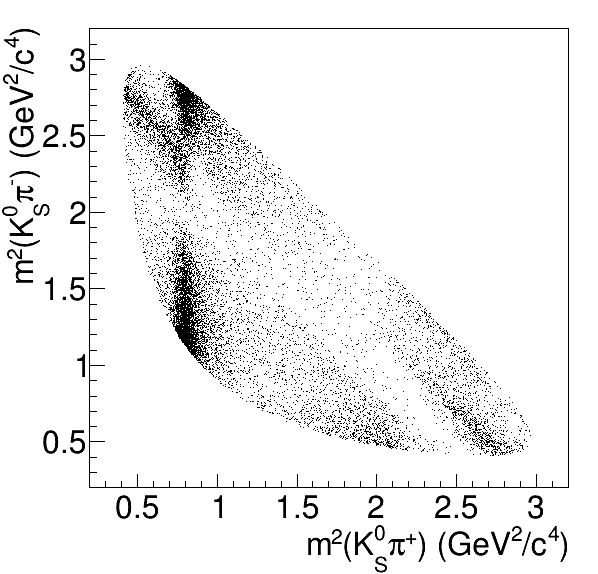
\includegraphics[width=\textwidth]{bp_dp_sig2}
  \subcaption{}
  \label{fig:bp_dp_sig}
 \end{minipage}
 \begin{minipage}[b]{0.5\textwidth}
  \centering
  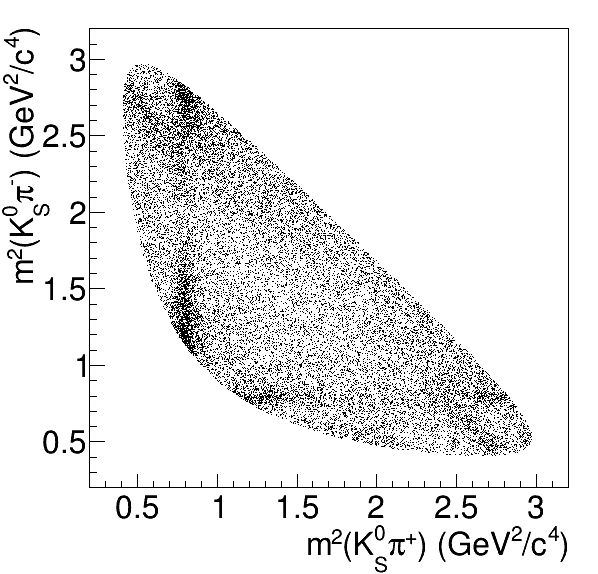
\includegraphics[width=\textwidth]{bp_dp_bkg2}
  \subcaption{}
  \label{fig:bp_dp_bkg}
 \end{minipage}
  \caption{Диаграммы Далица распада \dnkpp для $D$-мезонов, реконструированных в распадах \bpdpi для а) сигнальной и б) фоновой \de-\mbc областей.}
\label{fig:bpdpi_dp}
\end{figure}


Для измерения параметра \ki необходимо определить относительную вероятность попадания события в $i$-ю область диаграммы Далица:
\begin{equation*}
 K_i = \frac{N_i-B_i}{S},
\end{equation*}
где $N_i$ --- количество событий в $i$-й области диаграммы Далица, $B_i$ --- количество фоновых событий в этой области и $S$ --- полное количество сигнальных событий.

Для оценки распределения фоновых событий используется распределение Далица в фоновой области (рисунок~\ref{fig:bp_dp_bkg}), определенной как объединение двух областей:
\begin{equation}\label{eq:sideband}
\begin{split}
 &\mbc\in(5.23\gevcsq, 5.26\gevcsq)\ \cap\ \de\ \in\ (-0.15\gev, 0.30\gev),\\
 &\mbc\in(5.26\gevcsq, 5.29\gevcsq)\ \cap\ \de\ \in\ (\phantom{-}0.12\gev, 0.30\gev).
\end{split}
\end{equation}
Из-за малости доли фоновых событий, отличие фоновых распределений в сигнальной и фоновых областях не учитывалось.

Результат измерения параметров \ki приведен в таблице~\ref{tab:Kmeasured}.  Эти значения используются для измерения параметра~\pphi.

\begin{table}[htb]
\centering
 \caption{Величины параметров \ki, измеренные в распадах \bpdpi, \dbkpp.  Поправка на эффективность регистрации не выполнялась.}
 \label{tab:Kmeasured}
 \begin{tabular}
  { @{\hspace{0.7cm}}c@{\hspace{0.7cm}} @{\hspace{0.7cm}}r@{\hspace{0.7cm}} @{\hspace{0.7cm}}r@{\hspace{0.7cm}}}
  \hline\hline
   $i$ & \multicolumn{1}{c}{\ki (\%)} & \multicolumn{1}{c}{\kmi (\%)}\\ \hline
   $1$ & $17.42\pm0.32$ & $7.81\pm0.25$ \\% \hline
   $2$ & $ 7.51\pm0.22$ & $1.29\pm0.10$ \\% \hline
   $3$ & $10.24\pm0.26$ & $2.58\pm0.14$ \\% \hline
   $4$ & $ 2.85\pm0.14$ & $1.16\pm0.10$ \\% \hline
   $5$ & $ 9.45\pm0.25$ & $4.25\pm0.17$ \\% \hline
   $6$ & $ 7.31\pm0.22$ & $1.73\pm0.11$ \\% \hline
   $7$ & $10.48\pm0.26$ & $1.18\pm0.10$ \\% \hline
   $8$ & $12.46\pm0.28$ & $2.38\pm0.14$ \\ \hline
  \hline
 \end{tabular}
\end{table}

\section{Изучение распределения \dt}\label{sec:time_likelihood}
Параметр \pphi измеряется с помощью метода максимального правдоподобия, используя распределение по параметру \dt (разности времен распада сигнального и помечающего $B$-мезонов).  Функция правдоподобия определена следующим образом:
\begin{equation}\label{eq:lh}
 \mcl(\pphi) = \prod\limits_{j=1}^{N}\left[\fsigj\psig(\dtj,\pphi)+(1-\fsigj)\pbkg(\dtj)\right],
\end{equation}
где суммирование ведется по всем событиям в выборке, \psig обозначает плотность вероятности для сигнальных событий, \pbkg обозначает плотность вероятности для фоновых событий, \fsigj определена в уравнении~\eqref{eq:fsig_event-dependent} и обозначает вероятность того, что $j$-е событие является сигнальным.

\subsection{Параметризация фонового распределения \dt}
При описании распределений \dt необходимо учитывать, что пространственное разрешение при реконструкции вершин распадов в значительной степени зависит от \svd и отличается для данных, набранных с первой и второй версиями этого детектора ($\svd1$ и $\svd2$).  Распределения по \dt для фоновых событий описываются независимо для этих двух случаев.

Пространственное разрешение также существенно отличается для вершин, реконструированных посредством проецирования траектории единственного трека на область взаимодействия пусков и вершин, реконструированных с использованием нескольких треков.  Распределение по \dt для фоновых событий описывается независимо для вершин \brec, восстановленных с помощью одного трека (\emph{однотрековые вершины}), и вершин, восстановленных из нескольких треков (\emph{многотрековые вершины}).

С помощью событий общего моделирования установлено, что распределения фоновых событий по \dt в сигнальной и фоновой \de-\mbc областях существенно отличаются.  Поэтому подход, при котором фоновое распределение \dt определяется по событиям из фоновой области, а затем применяется для описания фона в сигнальной области, в базовом виде в данном случае применять не следует.

Однако, распределения \dt для фоновых \qqbar-событий и \bbbar-событий по отдельности почти не зависят от \de и \mbc.  Различие фоновых распределений \dt в сигнальной и фоновой областях возникает из-за изменения соотношения \qqbar- и \bbbar-компонент.  Принимая это наблюдение во внимание, фоновые распределения \dt описаны функцией 
\begin{equation}
 \pbkg\lbr \dt \rbr = \fqqj\pbkg^{(\qqbar)} + \lbr 1-\fqqj \rbr \pbkg^{(\bbbar)},
\end{equation}
где $\pbkg^{(\qqbar)}$ обозначает плотность вероятности для \qqbar-событий, $\pbkg^{(\bbbar)}$ обозначает плотность вероятности для \bbbar-событий и \fqqj обозначает долю \qqbar-событий в фоне, определенную аналогично~\eqref{eq:fsig_event-dependent}.

Оба распределения $\pbkg^{(x)}$, $x = \qqbar, \bbbar$ имеют вид
\begin{equation}
 \pbkg^{(x)}\lbr \dt_j\rbr = \int\limits_{-\infty}^{\infty} \lbr f^{(x)}_{\delta}\delta(\dt^{\prime})+\lbr 1-f^{(x)}_{\delta}\rbr 2\tbkg^{(x)} e^{-\frac{|\dt^{\prime}|}{\tbkg^{(x)}}}\rbr G^{(x)}_2\lbr\dt_j-\dt^{\prime}\rbr d\dt^{\prime},
\end{equation}
где $\delta$ обозначает дельта-функцию Дирака и $G_2$ обозначает сумму двух нормальных распределений с общим центральным значением:
\begin{equation}
 G^{(x)}_2\lbr \dt_j \rbr = f\subpeak^{(x)} G\subpeak\lbr\dt_j,\dt^{(x)}_0,s\subpeak^{(x)}\sigma_j\rbr+\lbr1-f\subpeak^{(x)} \rbr G\subtail\lbr\dt_j,\dt^{(x)}_0,s\subtail^{(x)}\sigma_j\rbr.
\end{equation}
Параметр $\sigma_j = \sqrt{\sigma_{\rec,j}^2+\sigma_{\asc,j}^2}$ определяется для каждого события из процедуры восстановления вершин распадов \brec и \basc.  Параметры функции \pbkg для каждого класса событий определяются с использованием событий общего моделирования.

При обработке экспериментальных данных в \pbkg вносятся поправочные параметры $\nu_1$ и $\nu_2$:
\begin{equation}\label{eq:dt_bkg_corrections}
 s^{(x)}_{\{{\tail},{\peak}\}} \to \nu_1 s^{(x)}_{\{{\tail},{\peak}\}},\quad
 \dt_0^{(x)} \to \dt_0^{(x)} + \nu_2.
\end{equation}
Значения параметров $\nu_1$ определяются с помощью анализа \dt распределений в фоновой области.  Эти значения определяются независимо для $\svd1$ и $\svd2$ и используются для всех сигнальных процессов:
\begin{equation}\label{eq:dt_bkg_scale_shift}
\begin{split}
 &\svd1:\quad \nu_1 = 1.20 \pm 0.06,\quad \nu_2 =          - 0.03 \pm 0.06 \ps,\\
 &\svd2:\quad \nu_1 = 1.25 \pm 0.03,\quad \nu_2 = \phantom{-}0.01 \pm 0.02 \ps.
\end{split}
\end{equation}

% \begin{figure}[htb]
%  \centering
%   \includegraphics[width=0.7\textwidth]{sidebandlin_m0}
%   \caption{Распределение \dt в фоновой области для процессов \bdsth.  Черные точки с ошибками показывают данные, непрерывная синяя линия показывает аппроксимацию. В нижней части показаны отклонение аппроксимации от данных, нормированное на статистическую ошибку.}
% \label{fig:dt_sideband}
% \end{figure}

На рисунке~\ref{fig:dt_sideband} показано аппроксимированное с помощью описанной процедуры распределение \dt в фоновой области для процессов~\bdsth.

\begin{figure}[htb]
 \centering
 \begin{minipage}[b]{0.45\textwidth}
  \includegraphics[width=\textwidth]{sidebandlin_m0}
  \subcaption{}
  \label{fig:dt_sideband}
 \end{minipage}
 \begin{minipage}[b]{0.45\textwidth}
  \includegraphics[width=0.92\textwidth]{lifetime_m0}
  \subcaption{}
  \label{fig:dt_lifetime}
 \end{minipage}
  \caption{Распределение \dt в а) фоновой и б) сигнальной областях для процессов \bdsth.  Черные точки с ошибками показывают данные, непрерывные синие линии показывают аппроксимацию, пунктирная синяя линяя показывает аппроксимацию сигнальной компоненты, пунктирная красная линия показывает аппроксимацию фоновой компоненты. В нижней части рисунков показано отклонение аппроксимации от данных, нормированное на статистическую ошибку.  Для наглядности, показаны только события в интервале~$[-10\ps, 10\ps]$, хотя анализ выполнен в интервале~$[-70\ps, 70\ps]$.}
\label{fig:dt_bdh}
\end{figure}

\subsection{Параметризация временного разрешения}\label{sec:time-resolution}
Функция $\psig(\dt)$, описывающая плотность вероятности распределения \dt для сигнальных событий, имеет следующий вид:
\begin{equation}\label{eq:psig_dt_cpv}
 \psig(\dt) = \int\limits_{-\infty}^{\infty}\mcp\subsig(\dtp)\mcr(\dt-\dtp)d\dtp,
\end{equation}
где $\mcp\subsig$ определена в уравнении~\eqref{eq:master-formula} и \mcr обозначает функцию разрешения.

Релятивистский фактор $\bgups=0.425$ рожденного в коллайдере KEKB \ups-резонанса определяет характерный отлет $B$-мезона $\beta c\btau\approx 180\mum$.  Величина этого отлета близка к характерной величине пространственного разрешения при реконструкции вершин распадов $B$-мезонов.  Поэтому понимание факторов, влияющих на пространственное разрешение и точное описание разрешения $\mcr(\dt)$ являются необходимыми условиями для выполнения времязависимых измерений с детектором Belle.  Функция $\mcr(\dt)$ учитывает:
\begin{itemize}
 \item Детекторное разрешение, которое определяется ошибками измерения импульсов и координат частиц в подсистемах детектора;
 \item Ошибки из-за вторичных вершин в цепочке распада \brec;
 \item Искажение распределения \dt из-за использования кинематического приближения~\eqref{eq:kine-appr}.% $\dt = \Delta z/(c\beta\gamma)$.
\end{itemize}
Явный вид функции разрешения $\mcr\lbr\dt\rbr$ приведен в приложении~\ref{app:time-resolution}.

\subsection{Измерение времени жизни $B$-мезона}
Время жизни нейтральных $B$-мезонов \btau измерено в распадах \bdsth (таблица~\ref{tab:data_lifetime}).  Полученные для разных групп событий значения \btau согласуются с известным значением $\btau^{\textrm{(PDG)}} = (1.519 \pm 0.005)\ps$~\cite{pdg}.  Основной целью данного измерения является проверка корректности описания фонового распределения \dt и временного разрешения для сигнальных событий. Сигнальное распределение описывается функцией
\begin{equation}\label{eq:psig_dt_lifetime}
 \psig^{\textrm{(notag)}}(\dtj) = \frac{1}{2\btau}\int\limits_{-\infty}^{\infty}\bexpp\mcr(\dtj-\dtp)d\dtp,
\end{equation}
которая получена из функции~\eqref{eq:psig_dt_cpv} усреднением по аромату $B$-кандидата $q_B$ и суммированием по всем областям диаграммы Далица.

\begin{table}[H]
\centering
\caption{Результаты измерения времени жизни нейтральных $B$-мезонов в процессах \bdsth.  Приведена только статистическая ошибка.  Асимметричные доверительные интервалы получены с помощью пакета~\textrm{Minos}~\cite{minos}.}
\label{tab:data_lifetime}
\begin{tabular}
{ @{\hspace{0.5cm}}l@{\hspace{0.5cm}} @{\hspace{0.5cm}}c@{\hspace{0.5cm}} } \hline\hline
Группа событий                            & \btau (\textrm{пс})\\ \hline 
\bdpi                                    & $1.537^{+0.120}_{-0.112}$ \\
\bdetagg                                 & $1.301^{+0.293}_{-0.260}$ \\
\bdetappp                                & $1.160^{+0.329}_{-0.269}$ \\
\bdomega                                 & $1.483^{+0.175}_{-0.160}$ \\
\bdetap                                  & $1.226^{+0.365}_{-0.294}$ \\
\bdstpi                                  & $1.156^{+0.233}_{-0.213}$ \\
\bdsteta                                 & $1.925^{+0.491}_{-0.401}$ \\\hline
Процессы с однотрековой вершиной \brec   & $1.516^{+0.099}_{-0.094}$ \\
Процессы с многотрековой вершиной \brec  & $1.408^{+0.141}_{-0.131}$ \\\hline
%All modes, w/  tag lepton                & $1.763^{+0.213}_{-0.188}$ \\
%All modes, w/o tag lepton                & $1.390^{+0.087}_{-0.084}$ \\\hline
Все процессы, $\svd1$                    & $1.502^{+0.231}_{-0.196}$ \\
Все процессы, $\svd2$                    & $1.480^{+0.088}_{-0.084}$ \\\hline
Все процессы                             & $1.483^{+0.081}_{-0.078}$ \\\hline
\hline
 \end{tabular}
\end{table}

% \begin{figure}[htb]
%  \centering
%   \includegraphics[width=0.7\textwidth]{lifetime_m0}
%   \caption{Распределение \dt в сигнальной области для процессов \bdsth.  Черные точки с ошибками показывают данные, непрерывная синяя линия показывает аппроксимацию, пунктирная синяя линяя показывает аппроксимацию сигнальной компоненты, пунктирная красная линия показывает аппроксимацию фоновой компоненты. В нижней части показано отклонение аппроксимации от данных, нормированное на статистическую ошибку.  Для наглядности, показаны только события в интервале $[-10\ps, 10\ps]$, хотя анализ выполнен в интервале $[-70\ps, 70\ps]$.}
% \label{fig:dt_lifetime}
% \end{figure}

Доля сигнальной компоненты \fsig для каждого события определяется из анализа \de-\mbc распределения.  Время жизни является единственным свободным параметром, значение которого определяется методом максимального правдоподобия при анализе распределения \dt в интервале $[-70\ps, 70\ps]$.  Распределение \dt для всех \bdsth событий из сигнальной области показано на рисунке~\ref{fig:dt_lifetime}.

%В таблице~\ref{tab:data_lifetime} приведены значения времени жизни \btau, измеренные с помощью различных групп событий.  
%Все значения согласуются с известным значением $\btau^{\textrm{(PDG)}} = (1.519 \pm 0.005)\ps$~\cite{pdg}.

%\begin{equation}
% \btau_{\textrm{PDG}} = (1.519 \pm 0.05)\ps.
%\end{equation}

%В качестве проверки корректности описания фонового \dt-распределения и временного разрешения для сигнальных событий, было измерено 

%\clearpage
\subsection{Измерение \cpconj-нарушающих параметров}\label{sec:cpv_results}
\cpconj-нарушающие параметры \sindbeta и \cosdbeta, рассматриваемые как независимые и неограниченные величины, получены методом максимального правдоподобия из распределений \dt.  Функция правдоподобия определена в уравнении~\eqref{eq:lh}.  Полученные значения для различных групп событий приведены в таблице~\ref{tab:data_cpv}.  Коэффициент корреляции между параметрами \sindbeta и \cosdbeta составляет примерно $-3\%$, поэтому точность измерения параметра \cosdbeta нельзя улучшить, зафиксировав значение параметра \sindbeta.  Малость коэффициента корреляции связана со значением параметров \ki, \ci и \si в различных областях диаграммы Далица: области, обладающие высокой чувствительностью к \sindbeta, почти не дают вклад в измерение \cosdbeta и наоборот.  Таблица~\ref{tab:data_cpv} (последний столбец) содержит также результаты измерений, в которых \sindbeta и \cosdbeta рассматривались как функции угла \pphi.  

На рисунке~\ref{fig:dp-bdh} приведены полученные распределения Далица распада \dkpp для процессов~\bdsth и~$\bnbar\to D^{*0}h^0$.

\begin{figure}[H]
\begin{minipage}[b]{0.5\textwidth}
  \centering
  \includegraphics[width=0.74\textwidth]{dp_bdh_b0}
  \subcaption{\bdsth}
\end{minipage}
\hfill
\begin{minipage}[b]{0.5\textwidth}
  \centering
  \includegraphics[width=0.74\textwidth]{dp_bdh_b0b}
  \subcaption{\bbdsth}
\end{minipage}
\caption{Распределения Далица распадов \dkpp для $D$-мезонов, рожденных в процессах а) \bdsth и б) $\bnbar\to D^{*0}h^0$.  Показаны события, для которых вероятность ошибки определения аромата \basc меньше $23\%$.}
\label{fig:dp-bdh}
\end{figure}

\begin{table}[htb]
\caption{Результаты измерения \cpconj-нарушающих параметров в процессах \bdsth.  Представлены результаты двух версий процедуры измерения. В первой версии параметры \sindbeta и \cosdbeta измерялись, как независимые параметры.  По второй версии измерялось значение угла \pphi. Приведена только статистическая ошибка.  Асимметричные доверительные интервалы получены с помощью пакета~Minos~\cite{minos}.}
\label{tab:data_cpv}
\begin{tabular}
{ @{\hspace{0.4cm}}l@{\hspace{0.4cm}} @{\hspace{0.4cm}}r@{\hspace{0.4cm}} @{\hspace{0.4cm}}r@{\hspace{0.4cm}} @{\hspace{0.4cm}}r@{\hspace{0.4cm}} } \hline\hline
Группа событий                & \sindbeta & \cosdbeta & \pphi (град) \\ \hline
\bdpi                         & $ 0.610^{+0.348}_{-0.367}$ & $0.879^{+0.463}_{-0.524}$ & $17.9^{+11.6}_{-10.7}$\\
%\bdetagg                      & $1.858^{+1.147}_{-1.223}$ & $0.9916^{+0.6744}_{-0.7522}$ \\
%\bdetappp                     & $2.855^{+1.253}_{-1.412}$ & $3.651^{+1.349}_{-2.189}$ \\
\bdomega                      & $-0.124^{+0.580}_{-0.558}$ & $1.276^{+0.615}_{-0.691}$ & $-2.6^{+15.5}_{-15.1}$ \\
%\bdetap                       & $0.4177^{+1.185}_{-1.525}$ & $-0.5965^{+3.163}_{-2.82}$ \\
%\btodstpi                     & $0.2118^{+0.9616}_{-0.9689}$ & $0.4105^{+1.178}_{-1.157}$ \\
%\btodsteta                    & $-2.086^{+1.287}_{-1.231}$ & $-0.4218^{+1.549}_{-1.084}$ \\\hline
Остальные процессы            & $ 0.443^{+0.486}_{-0.512}$ & $0.893^{+0.493}_{-0.546}$ & $13.2^{+15.0}_{-14.9}$ \\ \hline
Однотрековые вершины \brec    & $ 0.470^{+0.306}_{-0.317}$ & $0.807^{+0.377}_{-0.404}$ & $14.7^{+ 9.8}_{- 9.5}$ \\
Многотрековые вершины \brec   & $ 0.266^{+0.491}_{-0.499}$ & $1.417^{+0.556}_{-0.615}$ & $ 6.2^{+13.2}_{-12.6}$  \\\hline
%All modes, w/  tag lepton     & $ 0.773^{+0.362}_{-0.387}$ & $0.869^{+0.418}_{-0.472}$ & $ 21.6^{+11.9}_{-11.1}$ \\
%All modes, w/o tag lepton     & $ 0.114^{+0.365}_{-0.371}$ & $1.058^{+0.461}_{-0.477}$ & $ 3.1\pm10.5$  \\\hline
Все процессы, $\svd1$         & $ 0.167^{+0.653}_{-0.673}$ & $0.781^{+0.711}_{-0.750}$ & $ 5.6^{+22.1}_{-21.7}$ \\
Все процессы, $\svd2$         & $ 0.461^{+0.285}_{-0.291}$ & $1.032^{+0.346}_{-0.373}$ & $12.6^{+8.4}_{-8.2}$ \\\hline
Все процессы                  & $ 0.412^{+0.263}_{-0.267}$ & $0.973^{+0.309}_{-0.329}$ & $11.7^{+7.8}_{-7.7}$ \\\hline
\hline
 \end{tabular}
\end{table}

Обсуждение полученных результатов приведено в пункте~\ref{sec:cpv_discussion}.%, а сейчас переходим к обсуждению систематических неопределенностей измерения.

%\clearpage
\section{Оценка систематической неопределенности}\label{sec:systematics}
В этом разделе описаны источники систематических неопределенностей, присущие описываемому измерению \cpconj-нарушающих параметров.  Оценка систематических смещений \cpconj-нарушающих параметров $\delta\sindbeta$, $\delta\cosdbeta$ и $\delta\pphi$ выполнена несколькими способами, в зависимости от источника неопределенности.  

Влияние конечного импульсного разрешения и эффективности регистрации событий исследовано с помощью событий сигнального моделирования; неопределенность, связанная с описанием временного разрешения, оценена посредством варьирования параметров функции разрешения; влияние остальных источников неопределенности оценено с помощью введения дополнительных свободных параметров в функцию правдоподобия.

При введении дополнительных параметров \vecp, функция правдоподобия \mcl модифицируется следующим образом:
\begin{equation}\label{eq:nuislh}
 -2\log{\mcl_{\textrm{n}}} = -2\log{\mcl}+\sum\limits_{i,j}\left(p_i-p_i^{0}\right)\mck_{ij}\left(p_j-p_j^{0}\right),
\end{equation}
где $\vecp^0$ --- вектор центральных значений параметров \vecp, \mck --- обратная матрица ковариаций параметров \vecp (матрица \emph{концентраций}) и суммирование ведется по всем дополнительным параметрам.  Таким образом, предполагается, вектор параметров \vecp является набором случайных величин, подчиняющихся многомерному нормальному распределению.

Доверительные интервалы для полученных значений \cpconj-нарушающих параметров определены с помощью \emph{теста отношения правдоподобия}.  Отношение правдоподобия $\lambda$ для параметра $\xi$ определено следующим образом:
\begin{equation}\label{eq:confidence_intervals}
 \lambda(\xi)=\frac{\mcl(\xi,\hat{\hat{\vecp}})}{\mcl(\hat{\xi},\hat{\vecp})},
\end{equation}
где $\hat{\xi}$ --- значение параметра $\xi$, минимизирующее функцию правдоподобия, $\hat{\vecp}$ --- соответствующие значения параметров \vecp, $\hat{\hat{\vecp}}$ --- значения параметров \vecp, минимизирующие функцию правдоподобия для текущего значения $\xi$.  Границы доверительного диапазона $[\xi_{nl},\xi_{nr}]$, соответствующего $n$ стандартным отклонениям, определяются условием
\begin{equation}
 n^{2} = -2\log\lambda(\xi_{nl}) = -2\log\lambda(\xi_{nr}).
\end{equation}
Полученные таким образом доверительные интервалы соответствуют полной неопределенности измерения.  Систематическая неопределенность $\sigma^{\nuis}_{\pm}$ формально определяется как $\sigma^{\nuis}_{\pm} = \sqrt{\sigma_{\pm} - \sigma^{0}_{\pm}}$, где $\xi_{1r} = \hat{\xi} + \sigma_+$, $\xi_{1l} = \hat{\xi} - \sigma_-$, а $\sigma^{0}_{\pm}$ --- соответствующие положительные и отрицательные неопределенности, полученные при фиксированных параметрах \vecp.

Дополнительные параметры, которые использовались для оценки систематической неопределенности, описаны ниже.  Процедура измерения \cpconj-нарушающих параметров выполняется с использованием всего набора дополнительных параметров, поэтому систематическая неопределенность оценивается одновременно для нескольких источников.  Такая процедура позволяет учесть корреляции между различными источниками неопределенности.

\paragraph{Импульсное разрешение. }%\label{sec:syst-dp}
В разделе~\ref{sec:kinerec} обсуждалось, что кинематическая реконструкция с требованием на инвариантные массы \ks- и \dn-кандидатов позволяет значительно улучшить точность измерения параметров Далица.  После выполнения этой процедуры все же остаются события, для которых номер области диаграммы Далица определен неверно, что может привести к ошибке измерения параметров \cpconj-нарушения.

Этот эффект изучен с помощью событий сигнального моделирования.  На рисунке~\ref{fig:dp_confusion} приведены матрицы соответствия истинных и реконструированных номеров областей диаграммы Далица.  Благодаря применению кинематической реконструкции номер области верно восстанавливается для $\approx95\%$ событий.  

\begin{figure}[htb]
 \begin{minipage}[b]{0.45\textwidth}
  \centering
  \includegraphics[width=0.8\textwidth]{dbin_raw}
  \subcaption{}
 \end{minipage}
 \begin{minipage}[b]{0.49\textwidth}
 \hfill
  \centering
  \includegraphics[width=0.74\textwidth]{dbin_fit}
  \subcaption{}
 \end{minipage}
  \caption{Матрицы соответствия истинных и реконструированных номеров областей диаграммы Далица а) до и б) после применения алгоритма кинематической реконструкции с требованием на значения инвариантных масс \dn- и \ks-кандидатов.   Приведены значения (в \%), полученные с помощью событий сигнального моделирования процесса \bdpi.  Номер~$0$ реконструированной области означает, что событие лежит за пределами кинематически разрешенной области.}
  \label{fig:dp_confusion}
\end{figure}

Процедура определения \cpconj-нарушающих параметров была выполнена для событий сигнального моделирования с использованием восстановленных номеров областей.  Затем, для этих же событий была выполнена та же процедура, но с использованием истинных значений номеров областей.  Разности полученных значений \cpconj-нарушающих параметров
\begin{equation}
 \delta(\sindbeta) \approx 0.3\times10^{-2},\quad
 \delta(\cosdbeta) \approx 0.7\times10^{-2},\quad
 \delta(\pphi)     \approx 0.1\grad
\end{equation}
используются в качестве оценки систематической неопределенности, обусловленной импульсным разрешением.

\paragraph{Эффективность регистрации событий. }%\label{sec:syst-eff}
Зависимость эффективности регистрации событий от переменных Далица $\varepsilon(\mpsq,\mmsq)$, вообще говоря, может привести к смещению наблюдаемых значений параметров \ki, \ci и \si.  Для учета эффективности регистрации, в интегралах~\eqref{eq:ki} и \eqref{eq:csi} необходимо сделать замену
\begin{equation}
 \ddlz\to \varepsilon(\mpsq,\mmsq)\ddlz.
\end{equation}  

Если эффективность регистрации событий приводит к симметричным относительно отражения $\mpsq\leftrightarrow\mmsq$ преобразованиям вида
\begin{equation}
  K_i\to\alpha_i K_i,\quad K_{-i}\to\alpha_i K_{-i}\quad (\alpha_i>0),
\end{equation}
то смещения измеряемых параметров (смотрите уравнение~\eqref{eq:master-formula}) не возникает вовсе.  Этот факт позволяет ожидать подавления влияния эффективности регистрации событий.

Кроме того, поскольку значения параметров \ki измеряются в распадах \bpdpi, \dbkpp с кинематикой близкой к распадам \bdsth, \dbkpp, то можно ожидать существенное сокращение возможных поправок.

Наконец, возможное смещение параметров \ci и \si заведомо много меньше статистическая неопределенности для этих параметров, полученной в работе~\cite{CLEO_phases}.

Количественная оценка влияния эффективности регистрации событий на наблюдаемое значение параметра \pphi выполнено с помощью большой выборки событий сигнального моделирования.  После выполнения полной процедуры реконструкции для этих событий были взяты значения \dt генераторного уровня (истинные значения).  С помощью этих значений (и значений параметров \ki, \ci и \si, соответствующих модели распада, с помощью которой были сгенерированы события) были определены \cpconj-нарушающие параметры.  Полученные отклонения
\begin{equation}\label{eq:gen_offsets}
 \delta(\sindbeta) = (-5.5 \pm 4.3)\cdot 10^{-3},\quad\delta(\cosdbeta) = (-8.1 \pm 6.2)\cdot 10^{-3}
\end{equation}
от значений, использованных при генерации событий, согласуются с нулем.

\paragraph{Временное разрешение. }%\label{sec:syst-dt}
Неопределенность, связанная с описанием временного разрешения, оценивается с помощью варьирования параметров функции разрешения на величину стандартного отклонения в положительную и отрицательную стороны $\pm\sigma_{\pm}$.  Значения параметров, определенные с помощью событий моделирования, варьировались на два стандартных отклонения.  Параметры варьируются по одному, для каждого значения выполняется процедура определения \cpconj-нарушающих параметров.  Наибольшее отклонение полученного значения \cpconj-нарушающего параметра берется в качестве оценки неопределенности.  

Корень из суммы квадратов значений неопределенностей, полученных для каждого параметра функции разрешения, берется в качестве неопределенности, связанной с функцией временного разрешения: $\delta\sindbeta = 0.030$, $\delta\cosdbeta=0.066$ и $\delta\pphi = 0.1\grad$.

\paragraph{\boldmath Определение аромата $B$-мезона. }%\label{sec:syst-tag}
Неопределенность, связанная с процедурой определения аромата $B$-мезона, оценивается посредством добавления двух дополнительных параметров --- для событий $\svd1$ и $\svd2$.  Каждый параметр вносит общий сдвиг в вероятность неверного определения аромата для всех диапазонов параметра~$q$.

\paragraph{\boldmath Анализ распределений \de-\mbc. }%\label{sec:syst-dembc}
Для определения \cpconj-нарушающих параметров необходимо знать количество сигнальных событий в каждой области диаграммы Далица.  Количество сигнальных событий для всей выборки определяется с помощью анализа \de-\mbc распределения.  Количества сигнальных событий в каждой области диаграммы Далица (отдельно для \bn и \bnbar) определяются с помощью уравнения~\eqref{eq:nsig-prediction-with-tag}.  Это $2\times 16=32$ значения для каждого сигнального процесса.

Параметризация фонового распределения \dt использует долю фоновых \qqbar-событий, определенную с помощью анализа распределения \de-\mbc.  Для семи сигнальных процессов всего получается $33\times 7=231$ параметр.  Все эти параметры используются в качестве дополнительных параметров.  Получены следующие неопределенности, связанные с этими параметрами: $\delta\sindbeta = {}^{+0.038}_{-0.025}$, $\delta\cosdbeta={}^{+0.049}_{-0.026}$ и $\delta\pphi = 0.5\grad$.

\paragraph{\boldmath Параметризация фонового распределения \dt. }%\label{sec:syst-dtbkg}
Параметры, определенные в уравнении \eqref{eq:dt_bkg_corrections}, используются в качестве дополнительных параметров, соответствующих неопределенности, обусловленной описанием фонового распределения \dt. 

\paragraph{\boldmath Параметры \ki, \ci и \si. }%\label{sec:syst-kcs}
Параметры \ki, \ci и \si используются в качестве дополнительных параметров.  Для параметров \ci и \si используется матрица ковариаций, приведенная в дополнительных материалах к работе~\cite{CLEO_phases}.

Неопределенность в значениях параметров \ci и \si составляет доминирующий вклад в систематическую неопределенность измерения \cpconj-нарушающих параметров.

\paragraph{\boldmath Параметры \btau и \dmb. }%\label{sec:syst-taudm}
Время жизни нейтральных $B$-мезонов \btau и разность масс \dmb используются в качестве дополнительных параметров.  

В таблице~\ref{tab:systematics_cpv} приведены полученные оценки систематической неопределенности для каждого из описанных источников.

\begin{table}[H]
\caption{Систематические неопределенности измерения \cpconj-нарушающих параметров в распадах \bdsth.  Неопределенность $\sigma_{\textrm{nuis}}$ получена с помощью дополнительных параметров и соответствует источникам $4$--$10$.  Полная неопределенность $\sigma\subsyst$ определена, как $\sqrt{\sigma_1^2+\sigma_2^2+\sigma_3^2+\sigma_{\nuis}^2}$.  Величины $\sigma_4$--$\sigma_{10}$ приведены для иллюстрации.}
\centering
\label{tab:systematics_cpv}
\begin{tabular}
{ @{\hspace{0.2cm}}l@{\hspace{0.4cm}} @{\hspace{0.4cm}}c@{\hspace{0.4cm}} @{\hspace{0.4cm}}c@{\hspace{0.4cm}} @{\hspace{0.4cm}}c@{\hspace{0.2cm}} } \hline\hline
 Источник           & $\delta_{\sindbeta}$\,($\%$) & $\delta_{\cosdbeta}$\,($\%$) & $\delta_{\pphi}$\,(град)\\ \hline
1. Разрешение параметров Далица  & $0.3$           & $0.7$             & $0.1$ \\%MC
2. Эффективность регистрации     & $0.6$           & $0.8$             & $0.2$ \\%MC
3. Временное разрешение          & $3.8$           & $6.7$             & $1.2$ \\ %Standard
4. Определение аромата           & $0.1$           & $0.1$             & $<0.1$ \\
5. \dmb                          & $0.1$           & $0.1$             & $<0.1$ \\
6. \btau                         & $0.1$           & $0.1$             & $<0.1$ \\
7. Анализ распределений \mbc-\de & $3.4$           & $1.9$             & $0.8$ \\
8. Фоновое распределение \dt     & $3.6$           & $3.1$             & $0.7$ \\
9. \ki                           & $3.2$           & $2.0$             & $0.7$ \\
10. \ci и \si                    & $7.6$           & ${}^{+20}_{-13}$  & $1.1$ \\ \hline
$\sigma_{\nuis}$                 & $7.6$           & ${}^{+20}_{-13}$  & $1.6$ \\
Полная неопределенность $\sigma\subsyst$ & $8.5$           & ${}^{+21}_{-15}$  & $2.1$ \\
Стат. ошибка (для сравнения)     & $27$            & $33$              & $7.8$ \\ \hline
\hline
 \end{tabular}
\end{table}

\section{Обсуждение полученных результатов}\label{sec:cpv_discussion}
На рисунке~\ref{fig:lambda} показаны отношения правдоподобия, определенные в уравнении~\eqref{eq:confidence_intervals}, как функции \cpconj-нарушающих параметров. Результаты измерения, с учетом систематической неопределенности, следующие:
 \begin{equation}\label{eq:final_results}
 \begin{split}
  \sindbeta &= 0.43     \pm 0.27\stat    \pm 0.08    \syst,\\
  \cosdbeta &= 1.06     \pm 0.33\stat^{+0.21}_{-0.15}\syst,\\
  \pphi     &= 11.7\grad\pm 7.8\grad\stat\pm 2.1\grad\syst.
 \end{split}
 \end{equation}

Величина $\sindbeta=0.691\pm0.017$, измеренная в кварковых переходах \btoccs, определяет абсолютное значение \cosdbeta, которому соответствуют два значения угла $\pphi\in[0\grad; 180\grad)$.  Представленное в данной работе измерение исключает отрицательное значение \cosdbeta, соответствующее $\pphi = 68.1\grad$, на уровне $5.1$ стандартных отклонений и находится в согласии с положительным значением \cosdbeta, соответствующим значению $\pphi = 21.9\grad$ на уровне $1.3$ стандартных отклонений.  Таким образом, представленное измерение разрешает неопределенность в значении угла \pphi, присущую измерению параметра \sindbeta в переходах \btoccs.

\begin{figure}[htb]
 \begin{minipage}[b]{0.32\textwidth}
  \centering
  \includegraphics[width=\textwidth]{sin_minos_errors_v4}
  \subcaption{}
 \end{minipage}
 \begin{minipage}[b]{0.32\textwidth}
  \centering
  \includegraphics[width=\textwidth]{cos_minos_errors_v4}
  \subcaption{}
 \end{minipage}
 \begin{minipage}[b]{0.32\textwidth}
  \centering
  \includegraphics[width=\textwidth]{phi1_minos_errors_v4}
  \subcaption{}
 \end{minipage}
  \caption{Минус двойные логарифмы отношений вероятностей~$\lambda$~\eqref{eq:confidence_intervals} для а)~\sindbeta, б)~\cosdbeta и в)~\pphi. Черные квадраты (синие круги) показывают значения без учета (с учетом) систематических неопределенностей.  Черные пунктирные и синие непрерывные линии показывают аппроксимацию полученных значений.  Вертикальные красные линии показывают значения, соответствующие $\sindbeta=0.691$.  }
  \label{fig:lambda}
\end{figure}

Доминирующие систематические неопределенности могут быть уменьшены в измерениях с большей статистикой с данными эксперимента \belleii.  Действительно, неопределенности, обусловленные параметрами \ki, параметризацией временного разрешения и анализом распределений \de-\mbc, определяются размером выборки данных.  Параметры \ci и \si могут быть измерены более точно в эксперименте \besiii.

